\documentclass[aps,prl,twocolumn,groupedaddress]{revtex4-1}
\usepackage{graphicx}
\usepackage{amsmath}

\begin{document}
\title{Optical Pumping and Magnetic Resonance}
\author{Dongwon Han}
\author{Kevin Wood}
%\email[]{kevin.wood@stonybrook.edu}
%\thanks{}
\affiliation{Stony Brook University}

\date{\today}

\begin{abstract}
% insert abstract here
\end{abstract}

\maketitle

% body of paper here - Use proper section commands
% References should be done using the \cite, \ref, and \label commands
\section{Introduction}
%%%%%%%%%%%%%%%%%%%%%%%%%%%%%%%%%%%%%%%%
%%%%%%% Kevin is working on this %%%%%%%
%%%%%%%%%%%%%%%%%%%%%%%%%%%%%%%%%%%%%%%%
Rubidium (Rb) is an alkali metal with atomic number $Z=37$.
Neutral states contain four entirely filled electron shells with no net angular momentum and a single valence electron.
In its ground state, the valence electron carries no orbital angular momentum: $5^{2}S_{1/2}$.
In its first exited state, the valence electron carries one quanta of orbital angular momentum which can either align or anti-align with its spin contribution: $5^{2}P_{1/2}$ or $5^{2}P_{3/2}$. %"align or anti-align" probably isn't the best way to say this...
% I think that is okay. It is pretty clear what you meant to say

The energy splitting of the $5^{2}S$ and $5^{2}P$ states due to the Coulomb interaction with the nucleus is on the order of a few electron-volts.
% Isn't the pure Coulomb interaction between an electron and a nucleus completely determined by a principal quantum number n? In this case, both S and P states have n = 5. So orbital angular momentum must play role in this energy split.
The degeneracy of the first excited state is lifted by the spin-orbit coupling in which the electron's spin couples to the magnetic field set up by the positively charged nucleus in motion relative to the electron.
This effect introduces an energy gap that is on the order of $10^{-2}$ electron-volts between the $5^{2}P_{1/2}$ and $5^{2}P_{3/2}$ states.
A similar interaction between the nucleus and the magnetic field set up by the electron causes further energy splittings which are on the order of $10^{-9}$ electron-volts.
These energy levels are characterized by quantized z-component of the total, i.e. combined nuclear- and electron-, spin $m_{F}$ which couple to the magnetic field oriented in the z-direction.
It is this interaction that we will be probing by applying the techniques of optical pumping and magnetic resonance.

%overview of optical pumping
A Rubidium atom can transition between energy states by absorbing or emitting light.
When a single photon is absorbed by an Rb atom, conservation of angular momentum imposes a selection rule that limits which states are accessible.
By shining light of the appropriate energy onto a sample of Rb atoms, one can induce transitions from the ground state to the excited state.
The helicity of the light determines determines whether the quantum number $m_{F}$ will increase or decrease by one quanta per photon or remain constant.
These excited states can relax by emitting a photon and re-excite by absorbing yet another photon.
The relaxation process can increase, decrease, or not change $M_{F}$ at random depending on the helicity of the emitted photon; however, controlling the helicity of the incident light dictates which way the atom can become excited.
By continuing this process, all of the atoms in the sample will find themselves in either the maximal or minimal allowed $M_{F}$ state.
In this case, the sample is said to be \emph{optically pumped} into that quantum state and is unable to absorb any more of the light due to the lack of an excited state allowed by the selection rule.

%overview of magnetic resonance
By introducing an alternating magnetic field at a frequency corresponding to the hyperfine energy splitting, the Rb atoms are bathed in virtual photons with the correct energy to induce stimulated emission of real photons which relax the atom into a lower energy sublevel.
No longer in the maximal/minimal allowed $M_{F}$ state, the atom is not optically pumped and can once again absorb the incident light.
By sweeping different frequencies and monitoring the intensity of the transmitted light through a sample, one can probe the energy splittings that are artifacts of the atomic structure's finer details.

\section{Review of Previous Work}

\section{Experimental Set-up}

%%%%%%% DW is working on this %%%%%%%

The schematic of experimental design is shown in figure \ref{exp_schematic}.
We use a Rb discharge lamp and a lens to produce collimated Rb $D_1$ and $D_2$ lines.
We select circularly polarized D1 light by applying a spectral filter and a linear polarizer with a quarter wave plate.
The filtered light is focused at a heated Rb Cell, which contains both $^{85}Rb$ and $^{87}Rb$ isotopes.
The Rb cell also contains Argon (Ar) gas as a buffer.
%The buffer gas slows down the depolarization process by preventing Rb atoms hitting the wall too frequently.
The light emerges from the cell is refocused at a Si photodiode, which converts light to current.
The signal from the photodiode is amplified before recorded by LabView software.
%We use LabView software to collect and store data. 

\begin{figure}[h]
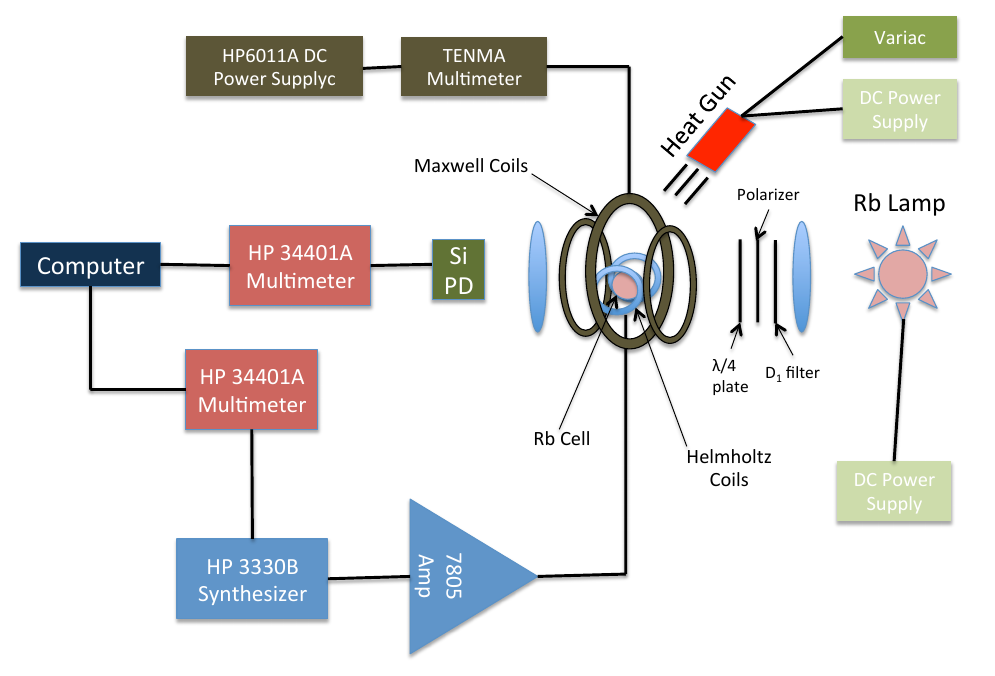
\includegraphics[width=\columnwidth]{exp_setup_schematic.png}
\caption{\label{exp_schematic}  Schematic of experimental setup}
\end{figure}

We use Maxwell coils to produce a uniform magnetic field around the Rb cell.
The entire apparatus is titled such that the center line of the apparatus is roughly parallel to the magnetic field of the Earth.
The Maxwell coils are arranged into the three coil configuration originally designed by James Clark-Maxwell in 1873.
This configuration enables us to convert DC current to a homogeneous magnetic field of known intensity.
The Maxwell coils are consisted of two smaller coils (labeled A and C) and one larger coil (labeled B).
Two smaller coils A and C are symmetrically placed with respect to coil B.
The displacement between the center of coil B and the center of smaller coil is $26.5\pm0.2$cm. 

The coils are wound with copper wire of known diameter, $0.132\pm0.005$cm.
The numbers of layers and turns per each layer is summarized in table \ref{maxcoil}.
The inner diameter of coil B is $78.4\pm0.5$cm, while those of coil A and C are $59.1\pm0.5$cm.
The Maxwell coils are shown in Figure \ref{exp_photo}.
A set of Helmholtz coils is placed orthogonal to the three Maxwell coils around the Rb cell.
These second set of coils are used to generate Radio Frequency (RF) field, which is controlled by a synthesizer.
We use the synthesizer to sweep various RF frequencies to locate the resonance peaks of $^{85}Rb$ and $^{87}Rb$ isotopes. 

\begin{figure}
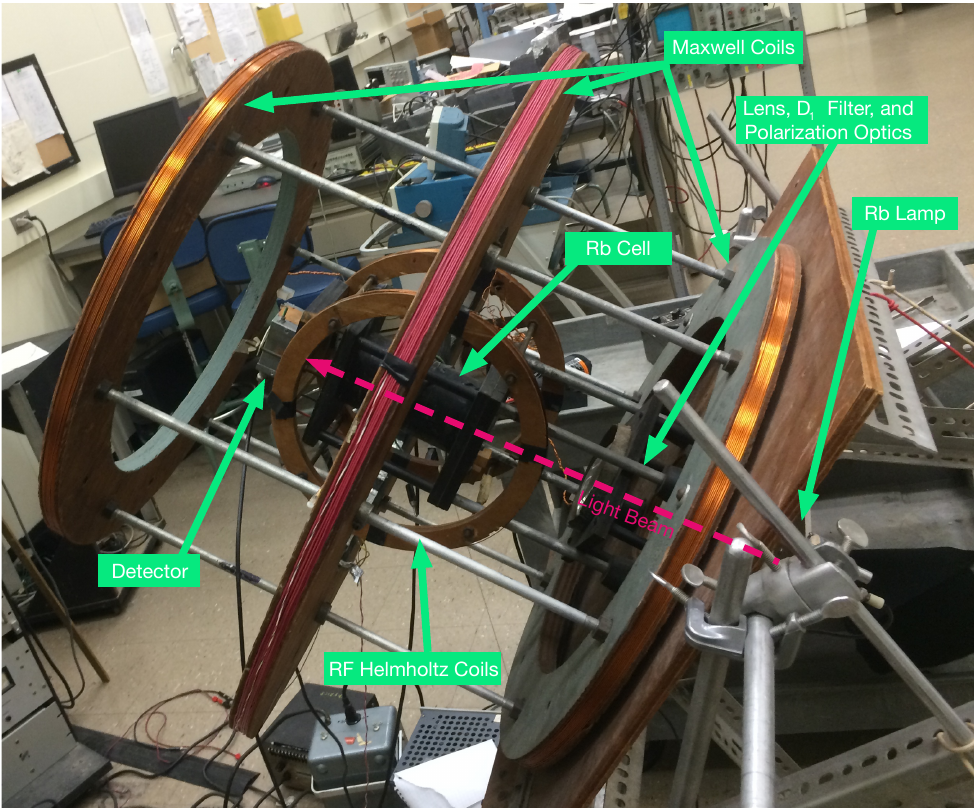
\includegraphics[width=\columnwidth]{exp_setup_photo.png}
\caption{\label{exp_photo} The optical pumping experiment apparatus}
\end{figure}

\section{Theoretical Model}
%%%%%%%%%%%%%%%%%%%%%%%%%%%%%%%%%%%%%%%%
%%%%%%% DW is working on this    %%%%%%%
%%%%%%%%%%%%%%%%%%%%%%%%%%%%%%%%%%%%%%%%

We first consider a atom with atomic number $Z$ orbited by $Z$ electrons. 
To the leading order, its energy levels are determined by Coulomb potential among the nucleus and electrons. 
Since the mass of the nucleus $M$ is much greater than that of electron $m_{e}$, i.e. $M \gg m_{e}$, we use Born-Oppenheimer (BO) approximation to separate the motion of the nucleus and electrons. In the rest frame of the nucleus, the following Hamiltonian describes the leading order interaction    

\small\begin{equation}\label{eq:leading_h}
\hat{H}_0 = \sum_{n=i}^Z \bigg(\frac{-\hbar^{2}}{2m_{e}}\nabla^{2}_{i} - \frac{1}{4\pi\epsilon_{0}}\frac{Ze^{2}}{r_{i}}\bigg) + \sum_{pairs ij}\frac{1}{4\pi\epsilon_{0}}\frac{e^{2}}{|r_{i}-r_{j}|} 
\end{equation}

The first term is a electron kinetic term. The second and third terms describe Coulomb interaction between the nucleus and a electron and among electrons respectively. 
In general, the third term is nonlinear and there is no analytic solution to this Hamiltonian.
Hydrogen like atom, which one studies in a elementary quantum mechanics course, is such special case. 
For a Hydrogen like atom, the solution to the equation \ref{eq:leading_h} and the corresponding energy levels are given by.

\begin{equation}\label{eq:leading_h_sol}
\psi_{nlm}(r,\theta,\phi) = R_{nl}(r)Y^{m}_{l}(\theta, \phi) 
\end{equation}

\begin{equation}\label{eq:leading_h_E}
E_{n} = \frac{-m_{e}c^{2}\alpha^{2}Z^{2}}{2n^{2}}
\end{equation}

where $\alpha$ is the fine structure constant, and $n$, $l$, and $m$ are quantum numbers described below.
To the leading order, the energy level of a Hydrogen like atom is solely determined by its radial quantum number n.
The other two quantum numbers l and m determine electron orbital momentum and the z component of electron orbital momentum respectively. 

We can use the solution and energy levels as a framework to describe more complex atoms like Rb.
The Pauli Exclusion principle forbids two identical fermions from occupying the same quantum state.
This allows us to``build up" a multi-electron solution by filling the lowest energy levels before filling the higher levels.
This idea is summarized in the Aufbau principle.

In this experiment, we use RB atoms which have 37 electrons.
Its full ground state configuration is $1s^{2}2s^{2}2p^{6}3s^{2}3p^{6}3d^{10}4s^{2}4p^{6}5s^{1}$.
Because the core electrons are "invisible" to our spectroscope, we can simplify our analysis by only considering single valence electron in $n=5$ state.

In the previous model, which only considers Coulomb interaction, energy levels are insensitive to electron spin, nuclear spin, and the z-component of the total angular momentum.
Each of them results in energy level degeneracy.   
In order to break this, we need to make a series of relativistic corrections to our Hamiltonian equation $\hat{H}_0$. 
In the weak magnetic field limit, under which this experiment is performed, they are spin-orbit coupling, hyperfine splitting, and Zeeman effect, listed from largest to smallest effect.

Spin-orbit coupling for $^{87}Rb$ is shown in figure \ref{fig:rb87_elevel}.
Spin-orbit coupling is due to the interaction between the spin of a electron and the magnetic field generated by a nucleus moving relative to it.
Depending on whether the electron spin "anti-aligns" with orbital angular momentum, energy levels either shift up or down. %% better way to say this?
In this experiment, spin-orbit coupling breaks $5P$ energy level degeneracy.
The energy of spin "aligned" state $5^2P_{1/2}$ is lowered, while that of "anti-aligned" state $5^2P_{3/2}$ is raised. 
Spin-orbit coupling is about 9 orders of magnitude smaller than Coulomb interaction. 
For Rubidium, the effect is about $0.03$ eV.  

\begin{figure}
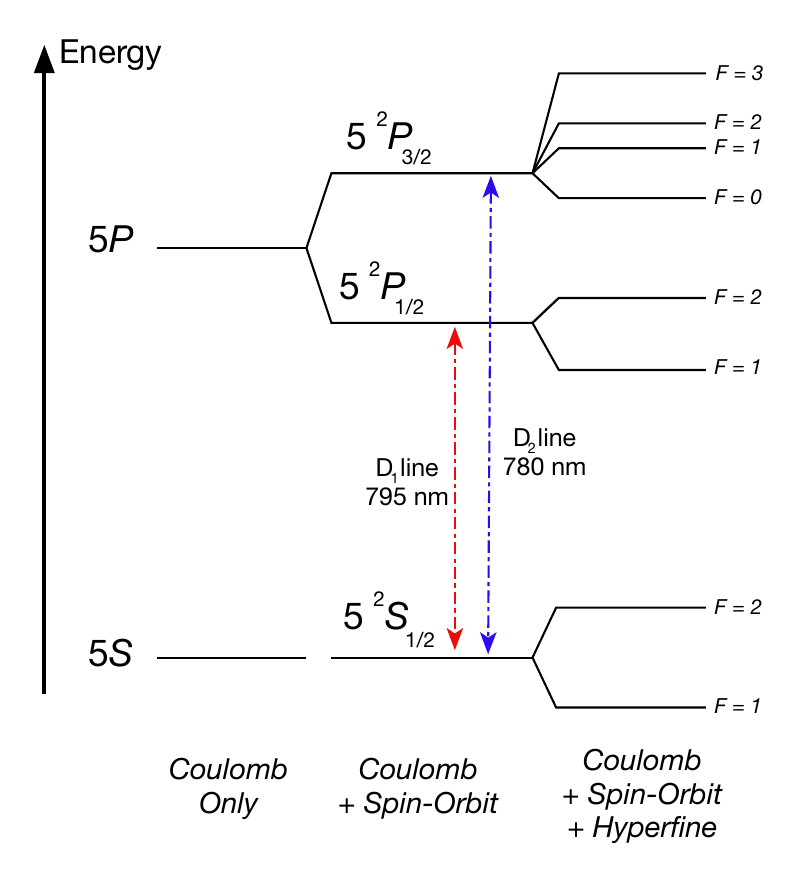
\includegraphics[width=\columnwidth]{Rb87_elevel_ver2.png}
\caption{\label{fig:rb87_elevel} Schematic diagram of $^{87}Rb$ energy levels }
\end{figure}

\subsection{Hyperfine Splitting}% for magnetic resonance explanation
The next order correction to our Hamiltonian is hyperfine splitting, which is due to the interaction of nuclear spin and the  magnetic field produced by electrons. 
In general, the interaction between a spin and magnetic field modifies Hamiltonian by 

\begin{equation}\label{eq:spin_magnetic_interaction_h}
\hat{H} = -\mu\cdot B
\end{equation}

In the case of hyperfine splitting, the relevant magnetic moment is the magnetic moment of nucleus $\mu_I$ and the magnetic field $B_{e}$ produced by electrons. 
For a nucleus with spin angular momentum I, its magnetic moment is given by the equation $\mu_I = g_{I}\mu_{N}I$. 
Here $\mu_N$ is the nuclear magneton and $g_{I}$ are the nuclear landau g-factor. 

Hyperfine splitting is described by a set of four quantum numbers, J, I, F, and $M_F$.
The total electron angular momentum number $J$ and nuclear spin number $I$,
along with the total angular momentum number $F = J + I$ and the z-component of the total angular momentum number $M_F$. 
Hyperfine energy levels are sensitive to the total angular momentum F. 
The hyperfine splitting of $^{87}Rb$ is shown in Figure \ref{fig:rb87_elevel}. 
In this experiment, the hyperfine splitting is about $10$ neV, which is about 6 orders of magnitude smaller than the spin-orbit effect. 

\subsection{Zeeman Effect}
We have lifted the energy level degeneracies by including the interaction between spins, electron and nuclear, with the internal magnetic fields. 
It remains to break the degeneracy due to the spherical symmetry of atom.
In the absence of a external field, a atom does not have a preferred direction, and its energy levels do not depend on a directionally dependent quantity. 
In particular, the hyperfine energy levels, shown in figure \ref{fig:rb87_elevel}, are insensitive to the z component of the total angular momentum. 
This leaves each hyperfine energy level $2F+1$ folds degenerate.
Zeeman effect is the breaking of this degeneracy by applying an external magnetic field.
In the weak field limit, Zeeman effect modifies our Hamiltonian by

\begin{equation}\label{eq:H_zeeman_weak_limit}
\hat{H}_{zeeman} = -g_F\frac{\mu_B B_{ext}}{\hbar} \hat{F}_{z}
\end{equation}   

where $g_F$ is the hyperfine landau g-factor. Zeeman effect of $^{87}Rb$ is shown in figure \ref{fig:rb87_elevel2}.

\begin{figure}
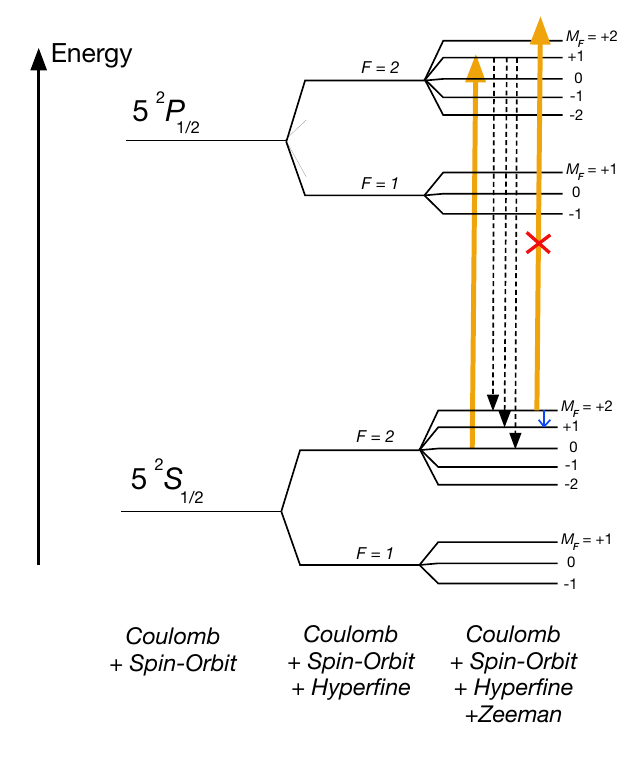
\includegraphics[width=\columnwidth]{Rb87_elevel.png}
\caption{\label{fig:rb87_elevel2} Schematic diagram of $^{87}Rb$ energy levels }
\end{figure}

In the strong B field limit, Zeeman effect is replaced with Paschen-Back effect. The physics behind both effects are the same. However, the Paschen-Back effect is larger than hyperfine splitting in this regime, and the good quantum numbers become j,l,s and i. Paschen-Back Hamiltonian is given by  

\begin{equation}\label{eq:H_zeeman_strong_limit}
\hat{H}_{PB} = -\frac{\mu_{B}B_{ext}}{\hbar}(g_J\hat{J}_z + g_I\hat{I}_z)
\end{equation}   

where $g_J$ and $g_I$ are the total electron and nuclear landau g-factors. In the intermediate regime, the solution is a linear combination of the weak field solution and the strong field solution. 

\subsection{Optical Pumping and Magnetic Resonance}
A atom can transition between energy states by absorbing or emitting a photon.
The conservation of angular momentum imposes a selection rule, which constrains the possible transitions between quantum states. The following lists describe the selection rule for a single photon transition.

\begin{itemize}
  \item Absorption: The total angular momentum increases by one quanta. The z-component of the total angular momentum either increases, decreases, or stay constant, depending on the helicity of the absorbed photon. 
  \item Emission: The total angular momentum decreases by one quanta. The z-component of the total angular momentum either increases, decreases, or stay constant, depending on the helicity of the emitted photon. 
\end{itemize}

In this experiment, we use Rb D1 light to excite Rb atom from S state to P state. Without the loss of the generality, we focus on the case where the absorbed photon has $\sigma^+$ helicity. 
As shown in figure \ref{fig:rb87_elevel2}, the ground state with $M_F = 2$ does not have an allowed exited states.
So once a Rubidium atom enters this state, it remains there.
As the excitation and relaxation process continue, more and more Rb atoms enters into the state.
Eventually, all Rb atoms are optically pumped into the state.

An alternating magnetic field at a frequency corresponding to the magnetic resonance frequency can cause a spontaneous emission of a photon. A Rubidium atom that goes through this process is no longer in the optically pumped state and can be excited again. In this experiment, we determine the magnetic resonance frequency by measuring this re-absorption signature.  

\section{Measurements}
%%%%%%%%%%%%%%%%%%%%%%%%%%%%%%%%%%%%%%%%
%%%%%%% Kevin is working on this %%%%%%%
%%%%%%%%%%%%%%%%%%%%%%%%%%%%%%%%%%%%%%%%
The optical pumping and magnetic resonance technique allows for a rich suite of measurements to probe the detailed atomic structure of relatively complicated elements.
Here we present measurements of the absorption cross-section of (optically pumped) Rubidium gas, the magnetic moments of the $^{85}\text{Rb}$ and $^{87}\text{Rb}$ isotopes, power broadening of the $^{85}Rb$ resonance peak, and hyperfine splitting.
\subsection{Rb Absorption Cross Section}
The absorption cross section of Rubidium was measured as the Rb cell warmed through the application of the Beer-Lambert law, which predicts the following relationship between the transmitted intensity of light and the number density of Rb atoms:
\begin{equation}\label{eq:beer}
I=I_{0}e^{-\sigma nl}.
\end{equation}
Here $I$ is the transmitted intensity, $I_{0}$ is the intensity of the incident light, $\sigma$ is the absorption cross section, $n$ is the number density of Rb atoms, and $l=0.05\text{ m}$ is the cell length.
The transmittance for a given Rb density was recorded via the photodiode, and the temperature of the cell was measured crudely with a mercury thermometer for each reading.
The monatomic Rubidium gas inside the cell is well-described by the ideal gas law
\begin{equation}\label{eq:idealgas}
n=\frac{N}{V}=\frac{P(T)}{k_{b}T}.
\end{equation}
At constant volume, the pressure of Rubidium gas as a function of temperature has been parameterized as the following:
\begin{equation}\label{eq:PofT}
P(T)=10^{4.857-4215/T}\text{ atm}
\end{equation}
where temperature $T$ is given in units of Kelvin.
Putting together Equations \ref{eq:idealgas} and \ref{eq:PofT} allows the determination of the Rb number density from the temperature measurements:
\begin{align}
n&=\left(\frac{101325.0\text{ Pa}}{1\text{ atm}}\right)\frac{(10^{4.857-4215/T}\text{ atm})}{(1.38\times10^{-23}\text{J/K})T}\\
&=1.006\times10^{33}\left(\frac{10^{-4214/T}}{T}\right)\text{ m$^{-3}$}
\end{align}
Figure \ref{RbXsection} shows the data from which the cross-section was calculated to be
\begin{equation}
\sigma=(6.06\pm0.06)\times10^{-17}\text{ m$^{2}$}.
\end{equation}

\begin{figure}
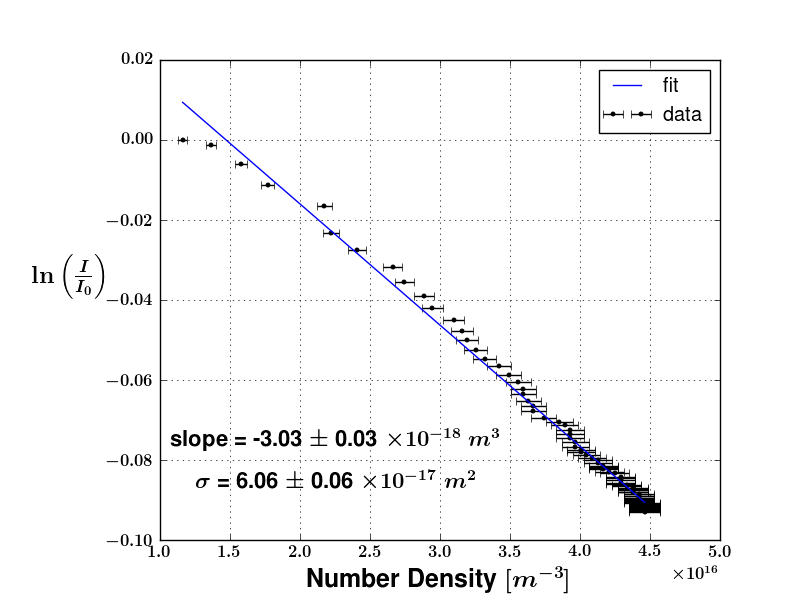
\includegraphics[width=\columnwidth]{rb-absorption-xsection.png}
\caption{\label{RbXsection} The absorption cross section of Rubidium  from the application of Beer-Lambert�s law to data taken as the Rb cell warmed.}
\end{figure}

\subsection{$^{85}$Rb and $^{87}$Rb Magnetic Moment}

When the sample is in an optically pumped state, it is unable to absorb the 795 nm D1 light from the heat lamp.
Consequently all of the light is transmitted and detected by the photodiode.
As the frequency of the alternating magnetic field set up by the Helmholtz coils approaches magnetic resonance, the atoms begin to drop from their optically pumped states and are thus able to absorb the D1 light.
In this case, the amount of transmitted light and therefore the photodiode reading will drop.
See Figure \ref{ResCurve} for an example of such a resonance curve.
By sweeping over a band of frequencies, one can deduce the energy splittings of the hyperfine structure by identifying the frequency which causes a drop in the photodiode signal and converting it to energy via
\begin{equation}
E=h\nu.
\end{equation}

The magnitude of this energy splitting is given by Equation \ref{eq:spin_magnetic_interaction_h}, which illustrates its linear dependence on the on the magnetic field present.
The proportionality factory, the nuclear magnetic moment $\mu_{I}$ was measured for both isotopes of Rb by varying the DC magnetic field with the Maxwell coils and finding the associated energy splitting.
Data from this procedure are shown in Figure \ref{MagMom}.

\begin{figure}[h]
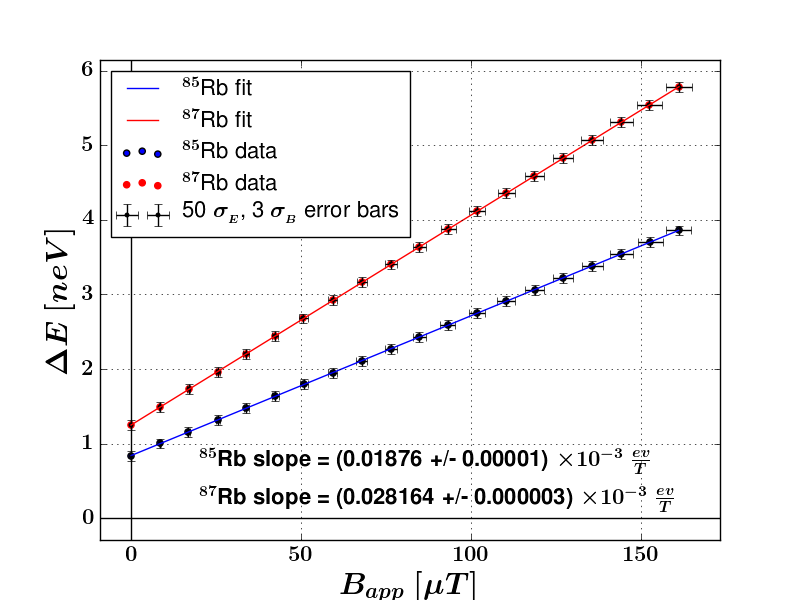
\includegraphics[width=\columnwidth]{magmom.png}
\caption{\label{MagMom} Measurement of the magnetic moment of $^{85}$Rb and $^{87}$Rb.}
\end{figure}

The error of the energy splitting for each data point was estimated by repeating the measurement 20 times for both no applied magnetic field and the maximum applied magnetic field of about 161 $\mu T$ and calculating the variance.
This showed that the absolute error, not the relative error, is what scales with the energy splitting and was determined to be $\sigma_{\Delta E}=0.0013$ neV (stat).
The error in the applied magnetic field arises from contributions from the uncertainties in the dimensions and positioning of the Maxwell coils as well as that of the current pushed through the coils.
$\sigma_{B}$ is field dependent and on the order of 1$\%$.
% refer to example frequency sweep in appendix
\subsection{Ambient Magnetic Field}

In the absence of an applied magnetic field as supplied by the Maxwell coils, there is an ambient field present due to the Earth's magnetic field, the atomic magnetic field, and any residual magnetic field from the laboratory equipment surrounding the experimental setup.
A measurement of this ambient field was performed by considering the energy splitting for no applied magnetic field in Figure \ref{MagMom}.

Applying Equation \ref{eq:H_zeeman_weak_limit} to the measured energy splittings of $^{85}$Rb and $^{87}$Rb under no applied field, the magnitude of the ambient field is found to be
\begin{equation}
B_{ambient}=42.717\pm0.075\, \mu T
\end{equation}
and
\begin{equation}
B_{ambient}=42.610\pm0.093\, \mu T,
\end{equation}
respectively.

The reported uncertainties are statistical in nature and are estimated by repeating the resonance sweep 20 times.
These measurements are consistent with one another and of the same order of magnitude as the magnetic field due to Earth at Stony Brook University, $B_{Earth}=51.704\, \mu T$, suggesting this is the main contribution to the ambient field. % ref: https://www.ngdc.noaa.gov/geomag-web/#igrfwmm 

\subsection{Power Broadening}

\begin{figure}[h]
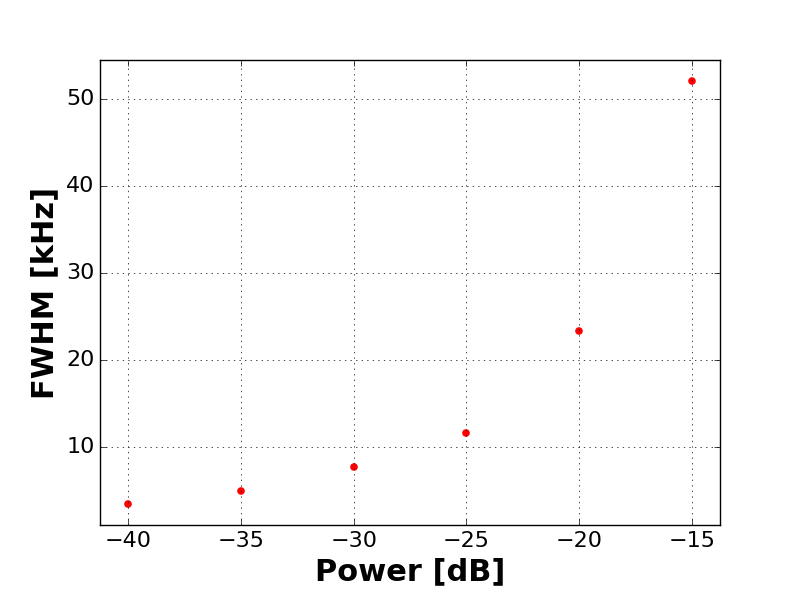
\includegraphics[width=\columnwidth]{powerbroad-rb85.png}
\caption{\label{PowerBroad} Power broadening of the $^85$Rb resonance peak.  The full width at half max (FWHM) of the resonance curve as a function of the Helmholtz coil.}
\end{figure}

\subsection{Hyperfine Splitting}

With a sufficiently high magnetic field, the magnetic resonance curves are sensitive to the particular $m_{F}$ quantum number of a given atomic state in addition to the change in $m_{F}$ from a transition.
In this field regime, one can observe multiple resonance peaks for a given isotope.
Figure \ref{HyperFineSplit} is an example of the hyperfine splitting of $^{85}$Rb under the presence of an applied $413$ $\mu T$ field.

\begin{figure}[h]
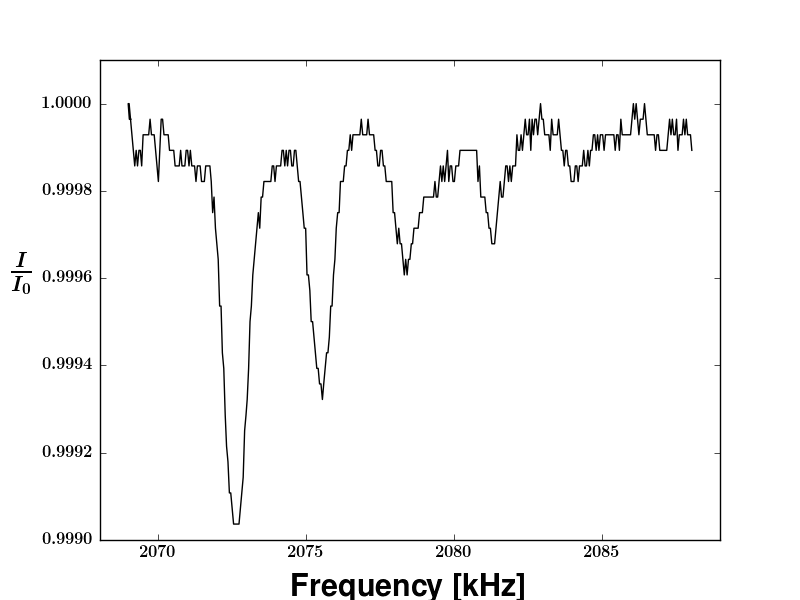
\includegraphics[width=\columnwidth]{rb85-hyperfine_split.png}
\caption{\label{HyperFineSplit} (data) Observation of hyperfine splitting of $^{85}$Rb.}
\end{figure}

The height of each peak is proportional to the differential occupation number, i.e. the difference between the occupation number of the initial and final states.
Figure \ref{HyperFineSplit} shows that the state corresponding to the lowest energy shift is most populated.
Furthermore, the non-linear behavior of the Breit-Rabi formula in the high-field regime predicts the energy spacing between two high $m_{F}$ states will be lower than that of two low $m_{F}$ states.% reference: http://home.sandiego.edu/~severn/p480w/OP_TW_5.pdf
It follows that the optically pumped state in this experiment was the (maximally valued) $m_{F} = +3$ state.
Clearly, the linear polarizer and quarter wave plate were set up to allow the right handed circular light ($\sigma_{+}$) to impinge the Rb cell.

\section{Comparison of Data and Theoretical Model}
%%%%%%%%%%%%%%%%%%%%%%%%%%%%%%%%%%%%%%%%
%%%%%%% Kevin is working on this %%%%%%%
%%%%%%%%%%%%%%%%%%%%%%%%%%%%%%%%%%%%%%%%
\section{Discussion and Conclusions}
\section{Author Contributions}
Both authors contributed to the data acquisition and analysis; however, the former was led by D. Han and latter by K. Wood.

D. Han wrote the ``Experimental Set-Up" and ``Theoretical Model" sections, while K. Wood wrote the ``Introduction" and ``Measurements" sections.
%Kevin: data analysis, "introduction", "measurements", "comparison of data and theoretical model",
%DW: data acquisition, "experimental set-up", "theoretical model"

%unclaimed: "Review of previous work", "discussion and conclusions"

\newpage
\appendix*
\section{Appendix}

\begin{table}[h]
\centering
\begin{tabular}{|c|ccc|}
\hline
Layer \#  & Coil A & Coil B & Coil C \\
\hline
1 & 11 & 11 & 11 \\
2 & 10 & 10 & 10 \\
3 & 11 & 11 & 11 \\
4 & 10 & 10 & 10 \\
5 & 11 & 11 & 11 \\
6 & 10 & 10 & 10 \\
7 & 11 & 11 & 11 \\
8 & 10 & 10 & 11 \\
9 & 11 & 11 & 11 \\
10 & 10 & 10 & 11 \\
11 & 5 & 11 & 3 \\
12 & 0 & 10 & 0 \\
13 & 0 & 11 & 0 \\
14 & 0 & 5 & 0 \\
\hline
\end{tabular}
\caption{\label{maxcoil} Number of layers and turns per each layer of three Maxwell coils}
\end{table}

\begin{figure}[h]
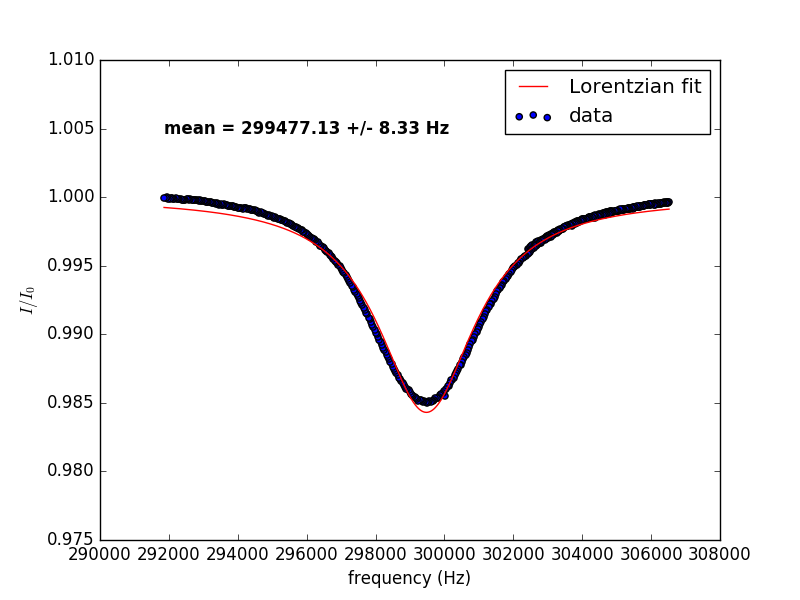
\includegraphics[width=\columnwidth]{rb85res-ambient-run1.png}
\caption{\label{ResCurve} Typical resonance curve.}
\end{figure}

\bibliography{basename of .bib file}

\end{document}